\feelchapter{Getting Started with Feel++}
            {Getting Started with Feel++}
            {Christophe Prud'homme, Baptiste Morin, Guillaume Dollé}
            {getting-started}


% first application
% (C) 2013 - Université de Strasbourg
% * Guillaume Dollé <guillaume.dolle@math.unistra.fr>
% * Christophe Prud'homme <christophe.prudhomme@feelpp.org>
% Tutorial documentation - myapp
%


\section{First \feel Application}
\label{sec:myapp}

See section \ref{sec:building} for more information about \feel installation.

\subsection{Minimal example}

Let's begin with our first program using the \feel framework
(source \textcolor{magenta}{"doc/manual/tutorial/myapp.cpp"}).
Before all, you have to include the \feel headers.
%
\vspace{2mm}
\begin{lstlisting}
  #include <feel/feel.hpp>
  using namespace Feel;
\end{lstlisting}
\vspace{2mm}
%
We use the C++ \lstinline!namespace! to avoid \lstinline!Feel::! prefix before
\feel objects.
%
\vspace{2mm}
\lstinputlisting[linerange=marker1-endmarker1]{tutorial/myapp.cpp}
\vspace{2mm}
%
\begin{itemize}
\item
We pass command line options using the
\href{http://www.boost.org/doc/libs/1_53_0/doc/html/program_options.html}
{Boost Program Options}\footnotemark[1] \lstinline!po::! library.
%
\footnotetext[1]{\url{http://www.boost.org/doc/libs/1_53_0/doc/html/program_options.html}}
%
To add a new \feel option, we must create a new
\feel \lstinline!options_description!. You must add the default \feel options
and the new one that we choose here as a double value. Note that the default
value will be assigned if not specified by the user.

\item
Then we initialize the environment variables through the \feel
\lstinline!Environment! class (Check the Constructor prototype on the online documentation).

\item
we instantiate a new application. We specify the directory where to execute the
program. That could be usefull for archiving your results.

\item
Finally, we save the results in a log file using the
\href{http://code.google.com/p/google-glog/}{google-glog library}
\footnotemark[2].
%
\footnotetext{\url{http://code.google.com/p/google-glog/}}
%
As you can see, we save in this example our custom option value and the
current processor number.

\end{itemize}


% \subsubsection{Advanced application}

% To integrate your application into the \feel framework, you will
% have to inheritate the super \lstinline!Application! class and to overload
% the \lstinline!run()! method.
% %
% \vspace{2mm}
% \begin{lstlisting}
% class MyApp : public Application
% {
%     public :
% 	void run();
% };
% \end{lstlisting}
% \vspace{2mm}
% %

\subsection{Compilation, execution, logs}

To compile a tutorial, just use the GNU make command.
%
\begin{unixcom}
    make feelpp_doc_<appname>
\end{unixcom}
%
where \textit{appname} is the name of the application you wish to
compile (here, \lstinline!myapp!).
Go to the execution directory as specified in the program,
and execute it. You can change your option value.
%
\begin{unixcom}
    ./feelpp_doc_myapp [--value 6.6]
\end{unixcom}
%
Now if you check the log,
%
\begin{unixcom}
    cat /tmp/<your login>/feelpp_doc_myapp/feelpp_doc_myapp.INFO
\end{unixcom}
%
you should see your value and the processor number used to compute.
You can run your application on several processors using MPI.
%
\begin{unixcom}
    mpirun -np 2 feelpp_doc_myapp
\end{unixcom}
%
Note that there will be one log for each processor in that case.


\subsection{Config files}

A config file can be parsed to the program to profile your options.
The default config paths are,
\begin{enumerate}
    \item current dir
    \item \verb|$HOME/feel/config/|
    \item \verb|$INSTALL_PREFIX/share/feel/config/|
\end{enumerate}
then you have to write inside one of these folders a file called
\lstinline!<app_name>.cfg! or \lstinline!feelpp_<app_name>.cfg!.
For example, our \lstinline!myapp.cfg! would looks like,
%
\vspace{2mm}
\begin{lstlisting}
    value=0.53
\end{lstlisting}
\vspace{2mm}
%
Note that you can specify the config file through the option \lstinline!--config-file=<path>!




\subsection{Initializing PETSc and Trilinos}

\index{PETSc}\index{Trilinos}\index{Libraries!PETSc}\index{Libraries!Trilinos}

PETSc is a suite of data structures and routines for the scalable (parallel)
solution of scientific applications modeled by partial differential
equations. It employs the MPI standard for parallelism.

\feel supports the PETSc framework, the \lstinline!Environment! \index{Environment}
takes care of initializing the associated PETSc environment.


% mesh manipulation
% (C) 2013 - Université de Strasbourg
% * Guillaume Dollé <guillaume.dolle@math.unistra.fr>
% * Christophe Prud'homme <christophe.prudhomme@feelpp.org>
% Tutorial documentation - mymesh
%


\section{Mesh Manipulation}
\label{sec:mymesh}

Feel++ provides some tools to manipulate mesh. 
Here is a basic example that shows
you how to generate a mesh for a square geometry
(source \textcolor{magenta}{"doc/manual/tutorial/mymesh.cpp"}).
%
\vspace{2mm}
\lstinputlisting[linerange=marker_main-endmarker_main]{tutorial/mymesh.cpp}
\vspace{2mm}

As always, we initialise the \feel environment (see section \ref{sec:myapp}).
The \lstinline!unitSquare()! will generate a mesh for a square geometry.
\feel provides several functions to automate the GMSH mesh generation
for different topologies.
%
( \lstinline!unitCircle()!,
  \lstinline!unitCube()!,
  \dots ).
%
These functions will create a geometry file
\textit{.geo} and a mesh file \textit{.msh}. We can visualize them in GMSH. 
%
\begin{unixcom}
    gmsh <entity_name>.msh
\end{unixcom}
%
Finally we use the \lstinline!exporter()! function to export the mesh for post processing.
It will create by default a \textbf{Paraview} format file \textit{.sos} and an \textbf{Ensight}
format file \textit{.case}.
%
\begin{unixcom}
    paraview <app_name>.sos
\end{unixcom}
%
For advanced usage, there is the more generic \lstinline!createGMSHMesh()! function which is
useful for creating or loading an existing mesh or geometry (see section \ref{howto:spec-meshes}
for a load example).
Note that \lstinline!unitSquare()! is just a particular case of \lstinline!createGMSHMesh()!.
\feel provide useful tools to iterate on the mesh or some faces that we will see later.
%
The process of the mesh creation is fully parallelized. You can as explained in section \ref{sec:myapp}
run this example on several processors and visualise subregions with paraview.




% integrals computing
% (C) 2013 - Université de Strasbourg
% * Guillaume Dollé <guillaume.dolle@math.unistra.fr>
% * Christophe Prud'homme <christophe.prudhomme@feelpp.org>
% Tutorial documentation - myintegrals
%

\section{Computing Integrals}
\label{sec:myintegrals}

You should be able to create a mesh now. If it is not the case, get back to the
section \ref{sec:mymesh}. This part explains how to integrate on a mesh with \feel
(source \textcolor{magenta}{"doc/manual/tutorial/myintegrals.cpp"}).
Let's consider the domain of the mesh,
\[
    \Omega=[0,1]^d=
    \{
        x\in\mathbb{R}^d\;,\;
        x_i>0\;
        \sum_{i=1}^d x_i \leqslant 1
    \}\in\mathbb{R}^d
\]
Here, we want to integrate the following function,
%
\begin{equation}
    f(x,y,z) = x^2 + y^2 + z^2
\end{equation}
%
on the whole domain $\Omega$ and on part of the boundary $\Omega$. Take a look at the code.
%
\vspace{2mm}
\lstinputlisting[linerange=marker_main-endmarker_main]{tutorial/myintegrals.cpp}
\vspace{2mm}
%
To use the \lstinline!integrate()! function, we have to precise the domain range. You can use,
\begin{itemize}
    \item \lstinline!elements()! to iterate on the whole mesh $\Omega$,
    \item \lstinline!boundaryfaces()! to iterate on the boundary $\partial\Omega$,
    \item \lstinline!markedfaces()! to iterate on a choose face.
\end{itemize}
%
You have to specify the expression we wish to compute. \feel provide a set of functions
to write these expressions \ref{sec:keywords}.
The \lstinline!evaluate()! function computes the integral on the global mesh.
The \lstinline!false! parameter limits the computation on the subregion owned by
the processor.
%
Note that \feel computes automatically the quadrature and consider by default each
non polynomial terms of the expression as a polynomial of degree 2. You can change
it by passing a \lstinline!_quad! parameter to the \lstinline!integrate()! function 
which takes a \lstinline!_Q<int order>! object as value.
(refer to API documentation).





% function spaces
[gmsh]
structured=1


[gmsh.domain]
shape=hypercube
convex=hypercube

[functions]
g=x*y*(y*2.2+4.3)*(2.1*x-1.3)


% solve laplacian dirichlet homogene
% (C) 2013 - Université de Strasbourg
% * Guillaume Dollé <guillaume.dolle@math.unistra.fr>
% * Christophe Prud'homme <christophe.prudhomme@feelpp.org>
% Tutorial documentation - mymesh
%


\section{Laplacian Problem}
\label{sec:tuto-mylaplacian}

This part explains how to solve the Laplacian equation 
for homogeneous dirichlet conditions,
%
\begin{equation}
\left\{
\begin{array}{rcll}
    -\Delta u & = & f & \text{on}\;\Omega \;, \\
            u & = & 0 & \text{on}\;\partial\Omega \;,\\
\end{array}
\right.
\end{equation}
%
where $u\in\Omega$ is the unknown "trial" function and $\Omega$ the domain.
%
We multiply each part of the first equation by a "test" function $v\in H_0^1(\Omega)$ 
and we integrate the resulting equation on the domain $\Omega$,
%
\begin{equation}
-\int_\Omega \Delta u \cdot v = \int_\Omega f\cdot v
\end{equation}
%
We can integrate by parts this equation (Green Theorem) to obtain \underline{the variationnal
formulation},
%
\begin{equation}
\int_\Omega \nabla u \nabla v
-\underbrace{ \int_{\partial\Omega} \frac{\partial u}{\partial \vec n}\cdot v }_{= 0}
=\int_\Omega f \cdot v \;.
\end{equation}
%
where $\vec n$ denotes a normal vector to the boundary. We can rewrite this equation as,
%
\begin{equation}
a(u,v)=l(v)
\end{equation}
where $a$ is a bilinear form, continuous, coercive and $l$ a linear form.
Let's take a look at the \feel code
(source \textcolor{magenta}{"doc/manual/tutorial/mylaplacian.cpp"}).
We consider for this example $f=1$ constant.
%
\vspace{2mm}
\lstinputlisting[linerange=marker_main-endmarker_main]{tutorial/mylaplacian.cpp}
\vspace{2mm}
%
As you can see, the program looks very close to the mathematical formulation.
We use the \lstinline!form2()! function to define the bilinear form and \lstinline!form1()!
for the linear one. The gradient for the trial functions is declared with the \lstinline!gradt()!
expression where as \lstinline!grad()! is used for the test functions
(see all keywords \ref{sec:keywords}).
Note that we need to transpose the second vector to perform the scalar product.
To introduce the homogeneous dirichlet conditions on the boundary, we use the function
\lstinline!on()!. Once the variationnal formulation and the boundary conditions are set, we call
the solver with \lstinline!solve()!.








% solve stokes poiseuille flow
% (C) 2013 - Université de Strasbourg
% * Vincent Huber <vincent.huber@cemosis.fr>
% * Guillaume Dollé <guillaume.dolle@math.unistra.fr>
% * Christophe Prud'homme <christophe.prudhomme@feelpp.org>
% Tutorial documentation - mymesh
%

\section{Stokes Problem}
\label{sec:tuto-mystokes}

Let solve the stokes equation considering a Poiseuille flow profile. 
We have the following system of equations,
%
\begin{equation}
\left\{
\begin{array}{rcll}
-\mu\Delta \bf u + \nabla p & = & \bf f & \text{on}\; \Omega \;, \\
                \div(\bf u) & = & 0 & \text{on}\; \Omega \;, \\
                \bf u  & = & g & \text{on}\; \Gamma \;, \\
\end{array}
\right.
\label{eq:tuto-stk}
\end{equation}
%
where $u\in [H_g^1(\Omega)]^d$ denotes the flow speed, $p\in [L_0^2(\Omega)]$ the fluid pressure, $\mu$ the 
fluid viscosity.
The last boundary condition expresses a null pressure fixed
on the outlet. The Poiseuille profile on the boundary is,
%
\begin{equation}
g(x,y)=
\left(
\begin{array}{c}
 y(1-y) \\
 0      \\
\end{array}
\right)
\end{equation}
%
The method used to obtain the strong formulation is closed to the one used
for the laplacian (see section \ref{sec:tuto-mylaplacian}).
We multiply the first equation by a test function $v\in H^1(\Omega)$
and we integrate on the domain $\Omega$,
%
\begin{equation}
-\int_\Omega \mu \Delta \mathbf u \cdot \mathbf v
+\int_\Omega \nabla p \cdot \mathbf v
=\int_\Omega \mathbf f \cdot \mathbf v \;.
\end{equation}
%
Then we use the Green Formula on the first term and we rewrite the second one 
to get the following equation,
%
\begin{equation}
\left(
\int_\Omega \mu \nabla \mathbf u : \nabla \mathbf v
-\int_{\partial\Omega} \frac{\partial \mathbf u}{\partial \mathbf n} \cdot \mathbf v
\right)
+\int_\Omega ( \div(p \mathbf v) - p\div(\mathbf v ) )
=\int_\Omega \mathbf f \cdot \mathbf v \;.
\label{eq:tuto-stk-1}
\end{equation}
%
where $n$ denotes a normal vector on the boundary.
The divergence theorem (or Gauss's theorem) gives,
%
\begin{equation}
\int_\Omega \div(p \mathbf v) = \int_{\partial\Omega} p \mathbf v\cdot \mathbf n \;.
\label{eq:tuto-stk-gauss}
\end{equation}
%
We have to add a consistency terms to the equation (\ref{eq:tuto-stk-1}) to
guaranty the symmetry of the bilinear form.
This term is provided by the second equation (\ref{eq:tuto-stk}). We multiply this equation
by a test function $q\in L_2(\Omega)$ and we integrate on the domain $\Omega$,
%
\begin{equation}
\int_{\Omega} \div(\mathbf u) q = 0 \;,
\label{eq:tuto-stk-secondeq}
\end{equation}
%
Finally, we deduce from the equations (\ref{eq:tuto-stk-gauss}), (\ref{eq:tuto-stk-secondeq})
and after rearranging the integrals (\ref{eq:tuto-stk-1}) the variationnal formulation,
%
\begin{equation}
\int_\Omega \mu \nabla \mathbf u :\nabla \mathbf v
+\int_\Omega \left( \div(\mathbf u) q - p \div(\mathbf v) \right)
+
    \int_{\partial\Omega} \left( p \mathbf n - 
 \frac{\partial \mathbf u}{\partial \mathbf n}\right)
     \cdot \mathbf v
=\int_\Omega \mathbf f \cdot \mathbf v 
\label{eq:tuto-stk-varform}
\end{equation}
%
Let us suppose now that $(\mathbf v,q) \in [H_0^1(\Omega)]^d \times L_0^2(\Omega)$, the variationnal formulation leads to:
Find $(\mathbf{u},p)\in [H_g^1(\Omega)]^d\times L_0^2(\Omega)$ such that for all $(\mathbf{v},q) \in [H_0^1(\Omega)]^d \times L_0^2(\Omega)$
\begin{equation}
\int_\Omega \mu \nabla \mathbf{u} :\nabla \mathbf{v}
+\int_\Omega \left( \nabla\cdot\mathbf{u} q - p \nabla\cdot\mathbf{v} \right)
=\int_\Omega \mathbf{f} \cdot \mathbf{v}
\end{equation}
Or equivalently:
\begin{equation}
  a((\mathbf{u},p),(\mathbf{v},q)) = l((\mathbf{v},q))
\end{equation}
where $a$ is a bilinear form, continuous, coercive and where $l$ is a linear form.
Let's see the \feel code corresponding to this mathematical statement.
(source \textcolor{magenta}{"doc/manual/tutorial/mystokes.cpp"}).
We suppose for this example the viscosity $\mu=1$ and $\mathbf f = 0$.
%
\vspace{2mm}
\lstinputlisting[linerange=marker_main-endmarker_main]{tutorial/mystokes.cpp}
\vspace{2mm}
%

The procedure to create the mesh is very simple.
You have to provide to the command line (or via the cfg file) the gmsh.filename option.
You can provide a geo or a msh file (created via gmsh).

As for the laplacian problem, the code is very closed to the mathematical formulation.
We define the product of function spaces for the flow speed and the flow pressure
using \lstinline!THch<order>()~\footnote{TH stands for Taylor-Hoods;}! function which is \lstinline!Pch<N+1>!$\times$ \lstinline!Pch<N>!
for respectively flow speed and pressure spaces.
We take an element 
$U=\left(
    \begin{array}{c}
        u \\
        p \\
    \end{array}
\right)
$
in this space. Then we define the integrals of the variationnal formulation
for the left and the right hand side. Finally, we apply the Poiseuille profile on the boundary.
We call the solver to resolve the problem (\ref{eq:tuto-stk-2}).





% solve advection equations
% (C) 2013 - Université de Strasbourg
% * Guillaume Dollé <guillaume.dolle@math.unistra.fr>
% * Christophe Prud'homme <christophe.prudhomme@feelpp.org>
% Tutorial documentation - mymesh
%

\section{Diffusion advection reaction problem}
\label{sec:tuto-myadvection}

The diffusion advection reaction equation is a classical partial differential
equation which can be found in many processes for example in chemistry or
biology. This can be described by an equation containing a diffusion, an
advection and a reaction term as follows,
%
\begin{equation}
  \left\{
    \begin{array}{rcll}
      -\epsilon\Delta  u + \bbeta \cdot \nabla  u + \mu u & = & f & \text{on}\; \Omega \;, \\
      u  & = & 0 & \text{on}\; \partial\Omega \;, \\
    \end{array}
  \right.
  \label{eq:tuto-adv}
\end{equation}
%
We use here homogeneous Dirichlet boundary conditions.

\subsubsection{Variationnal formulation}

To establish the variationnal formulation, as always we mutiply the first equation by a
test function $v\in H_0^1(\Omega)$ such that,
\[
    H_0^1(\Omega) = \{ v\in H^1(\Omega),\; v=0 \; \text{on} \; \partial\Omega \} \;.
\]
Then we integrate on the domain $\Omega$,
%
\begin{equation}
- \int_\Omega \epsilon \Delta u\ v
+ \int_\Omega \bbeta \cdot \nabla u\ v
+ \int_\Omega \mu\ u\ v
= \int_\Omega f\ v \;.
\end{equation}
%
We establish the variationnal formulation from the previous equation and using
the Green formula, find $u \in \in H_0^1(\Omega)$
%
\begin{equation}
  \int_\Omega \epsilon \nabla u \cdot \nabla v
  - \underbrace{\int_{\partial\Omega} \epsilon (\nabla u \cdot \mathbf n)\ v}_{=0}
  + \int_\Omega (\bbeta \cdot \nabla u)\ v
  + \int_\Omega \mu\ u\ v
  = \int_\Omega f v \; \quad \forall v \in \in H_0^1(\Omega),
  \label{eq:tuto-adv-varform}
\end{equation}
%
where $\mathbf n$ is a unit outward normal vector. We can rewrite the problem,
find $u \in \in H_0^1(\Omega)$
%
\begin{equation}
    a(u,v) = l(v) \quad \forall v \in \in H_0^1(\Omega),
\label{eq:tuto-adv-bilform}
\end{equation}
%
where $a$ is a bilinear form, continuous, coercive and $l$ is a linear form.

\subsubsection{Application}

We choose for our example $\mu = 1$, $\epsilon = 1$, $f=1$, and
$\bbeta=(1,1)^T$.

%
\vspace{2mm}
\lstinputlisting[linerange=marker_main-endmarker_main, caption={\lstinline{doc/manual/tutorial/myadvection.cpp}}]{tutorial/myadvection.cpp}
\vspace{2mm}
%
Again the implementation is close to the mathematical formulation.  Here again,
we create the mesh for an unit square geometry. Then we define the function
space $X_h$ we choose as order 1 Lagrange basis function using
\lstinline!Pch<Order>()!.  Note that here, the function space is the same for
"trial" and "test" functions.  We declare the left and the right hand side
integrals expressions for the equation (\ref{eq:tuto-adv-varform}). Finally we
add the Dirichlet boundary condition and we use the default solver to solve
(\ref{eq:tuto-adv-bilform}).  We export the solution $u$ for post processing.



\begin{figure}[htbp]
  \centering
  \subfigure[$\epsilon=1$]{
\includegraphics[width=.3\linewidth]{pngs/myadvection/sol-dar-1.png}}
  \subfigure[$\epsilon=0.01$]{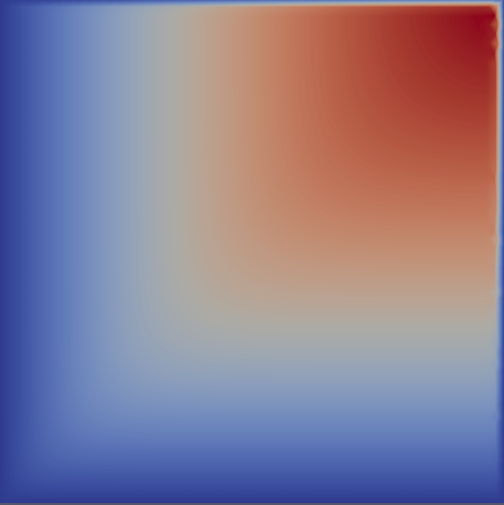
\includegraphics[width=.3\linewidth]{pngs/myadvection/sol-dar-2.png}}
  \subfigure[$\epsilon=0.0001$]{
\includegraphics[width=.3\linewidth]{pngs/myadvection/sol-dar-3.png}}
  \caption{Various solutions of problem~\eqref{eq:tuto-adv-bilform}  for $\epsilon=1,0.01,0.0001$. Notice how
  the solution gets unstable for $\epsilon=0.0001$, this is classical and
  requires stabilisation methods to handle this issue.}
  \label{fig:tut:1}
\end{figure}

%%% Local Variables:
%%% coding: utf-8
%%% mode: latex
%%% TeX-PDF-mode: t
%%% TeX-parse-self: t
%%% x-symbol-8bits: nil
%%% TeX-auto-regexp-list: TeX-auto-full-regexp-list
%%% TeX-master: "../feelpp-manual"
%%% ispell-local-dictionary: "american"
%%% End:



\section{Linear Algebra}
\label{sec:linear-algebra}

\feel supports \textsc{PETSc} as it Linear algebra backend. \textsc{PETSc} is a
suite of data structures and routines for the scalable solution of scientific
applications modeled by PDE available at
\url{http://www.mcs.anl.gov/petsc/petsc-as/}



\subsection{Choosing a linear algebra backend}
\label{sec:choos-line-algebra}

\index{Class!Backend}\index{boost!shared\_ptr}
To select a backend in order to solve a linear system, we instantiate
the \lstinline!Backend! class associated :
\begin{lstlisting}
#include <feel/feelalg/backend.hpp>
boost::shared_ptr<Backend<double> > backend =
     Backend<double>::build( BACKEND_PETSC );
\end{lstlisting}
The backend provides an interface to solve
\begin{equation}
  \label{eq:8}
  A x = b
\end{equation}
where $A$ is a $n \times n $ sparse matrix and $x,b$ vectors of size $n$. The backend defines the \cpp types for  each of these, e.g :
\begin{lstlisting}
Backend<double>::sparse_matrix_type A;
Backend<double>::vector_type x,b;
\end{lstlisting}
In practice, we use the \lstinline!boost::shared_ptr<>! shared pointer
to ensure that we won't get memory leaks. The backends provide a
corresponding \lstinline!typedef!

\begin{lstlisting}
Backend<double>::sparse_matrix_ptrtype A( backend->newMatrix( Xh, Yh ) );
Backend<double>::vector_ptrtype x( backend->newVector( Yh ) );
Backend<double>::vector_ptrtype b( backend->newVector( Xh ) );
\end{lstlisting}
where $X_h$ and $Y_h$ are function spaces providing the number of
degrees of freedom that will define the size of the matrix and vectors
thanks to the helpers functions \lstinline!Backend::newMatrix()! and
\lstinline!Backend::newVector!. In a parallel setting, the
local/global processor mapping would be passed down by the function
spaces.

%\subsection{Defining and using matrices and vectors}
%\label{sec:defin-using-matr}

\subsection{Solving}
\label{sec:solving}

To solve the linear problem $Ax=b$, the backend provides a function \lstinline!solve! with three required parameters
\begin{lstlisting}
 solve(_matrix=A, _solution=x, _rhs=b)
\end{lstlisting}
where :
\begin{itemize}
\item the matrix $A$ has a \lstinline!sparse_matrix_ptrtype! type
\item the solution $x$ has a type \lstinline!vector_type! or \lstinline!vector_ptrtype!
\item the second member vector $b$ has a type \lstinline!vector_ptrtype!
\end{itemize}
You can also add optional parameters like :
\begin{itemize}

\item a preconditioner : instead of solving $Ax=b$, we solve $P^{-1}Ax= P^{-1}b$. This method can be applied in iterative methods and permits to decrease the number of iterations in the resolution system

\item a maximum number of iterations : this option is used with an iterative solving method

\item a residual tolerance : the fraction $\displaystyle{\frac{\mid\mid r^{(k)} \mid\mid }{\mid\mid r^{(0)} \mid\mid}}$ is inferior to the residual tolerance with
$r^{(k)}=b-Ax^{(k)}$ and $x^{(k)}$ the solution at the $k^{th}$ iteration

\item a absolute tolerance : $\mid\mid r^{(k)} \mid\mid $ is inferior to the absolute tolerance

\item a different tolerance : sometimes, the residue doesn’t decrease continuously during the iterations. The difference between two plots doesn’t have to exceed the parameter choosen for the difference tolerance.

\item a boolean to use transpose matrix : instead of solving $Ax=b$, we solve $A^{t}x=b$. If $A$ is defined and positive, $A^{t}=A$.

\end{itemize}

To have a view of the values of the optional parameters, see the following code :

\begin{lstlisting}
BOOST_PARAMETER_MEMBER_FUNCTION(
	(solve_return_type),
         solve,
         tag,
         (required
	(matrix,(sparse_matrix_ptrtype))
	(in_out(solution),*(mpl::or_<boost::is_convertible<mpl::_,vector_type&>,
                                         boost::is_convertible<mpl::_,vector_ptrtype> >))
	(rhs,(vector_ptrtype)))
	(optional
	  (prec,(sparse_matrix_ptrtype), matrix )
	  (maxit,(size_type), 1000 )
	  (rtolerance,(double), 1e-13)
	  (atolerance,(double), 1e-50)
	  (dtolerance,(double), 1e5)
	  (reuse_prec,(bool), false )
	  (transpose,(bool), false )
	  )
	)
    {
\end{lstlisting}

\noindent The library \lstinline!Boost::Parameters! allows you to enter parameters in the order you want. It supports deduced parameters,  that is to say parameters whose identity can be deduced from their types.


